%\subsection{$\epsilon$ vs $\eta$ simulations}
%\clearpage
\subsection{Packing density vs shell potential simulations}

Basing on the previous studies of 2D systems\cite{stability,stability2} it can be concluded that
some interesting structures can self-assemble only in a small range of temperatures and packing densities. Besides, not all shell-to-core ratios contribute to the formation of the rotational order. Taking everything above into account subsequent simulations were performed at constant shell potential and packing density with three shell-to-core ratio values --- $\frac{2}{\sqrt[]{3}}=1.1547$, $\sqrt[]{2}=1.4142$, $\frac{\sqrt{8}}{3}=1.633$. The investigated regions are marked with dashed lines on the \textbf{Figure} \ref{fig:phase}. 

\subsubsection{The 1.1547 shell-to-core ratio}

The value of $\frac{2}{\sqrt[]{3}}=1.1547$ was chosen as it resembles the distance ratio between next-nearest and nearest neighbors in BCC.
The obtained results of the simulation are summarized as phase diagram in the \textbf{Figure} \ref{fig:phase_eta_eps}. As seen from the diagram three phases can be distinguished --- disordered liquid, hard-sphere FCC and BCC. 

\begin{figure}
\centering
\includegraphics[width=0.9\textwidth]{phase1_15_1.tikz}
\caption{Phase diagram packing density $\eta$ vs potential $\epsilon$ at constant $\lambda=1.1547$ with bond order diagrams of the formed phases} \label{fig:phase_eta_epssmall}
\end{figure}

\begin{figure}
\centering
\begin{subfigure}{.61\textwidth}
  \centering
  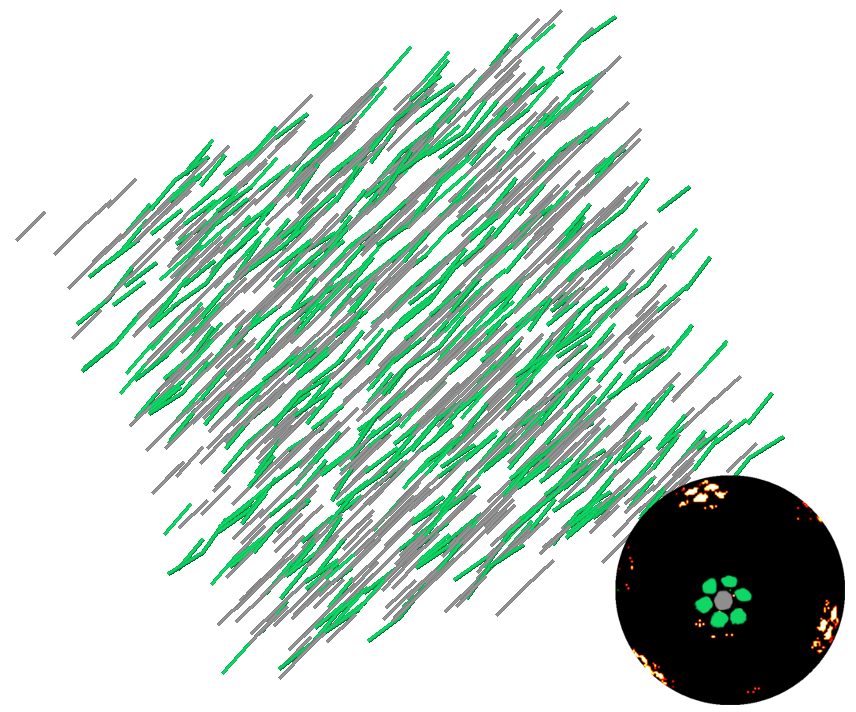
\includegraphics[width=0.98\textwidth]{bonds}
  \caption{}
  \label{fig:bondsmod} 
\end{subfigure}
\begin{subfigure}{.4\textwidth}
  \centering
 \includegraphics[width=0.95\textwidth]{upotmodBCC.tikz}
\caption{}
\label{fig:epot_modBCC} 
\end{subfigure}
\begin{subfigure}{.4\textwidth}
  \includegraphics[width=0.95\textwidth]{rdfmodul.tikz}
\caption{}% of the modulated BCC** phase, obtained at constant  $\lambda=1.1547$ and its deformed unit cell} 
\label{fig:rdfmodul}
\end{subfigure}
\caption{The BCC** structure describing parameters: \subref{fig:bondsmod} -- BCC** bonds distribution, \subref{fig:epot_modBCC} -- typical curve of the evolution of potential energy / $\epsilon$ vs time during the formation of BCC** structure and \subref{fig:rdfmodul} -- typical RDF shape}
\label{fig:modulaphase}
\end{figure}

%     \centering
%     \begin{minipage}{0.31\textwidth}
%         \centering
%         \includegraphics[width=0.95\textwidth]{upotmodBCC.tikz}
% \caption{Typical curve of the evolution of potential energy / $\epsilon$ vs time during the formation of BCC** structure at constant  $\lambda=1.1547$ }
% \label{fig:epot_modBCC}        
%     \end{minipage}\hfill
%     \begin{minipage}{0.45\textwidth}
%         \centering
%  \includegraphics[width=0.95\textwidth]{rdfmodul.tikz}
% \caption{Typical RDF shape of the modulated BCC** phase, obtained at constant  $\lambda=1.1547$ and its deformed unit cell} 
% \label{fig:rdfmodul} 
%     \end{minipage}
% \end{figure}

Modulated BCC** phase was observed at high values of packing density and shell potential.% and thus several simulations with higher than 0.53 packing density were performed. 
The part of the phase diagram where BCC** was observed is shown in the \textbf{Figure} \ref{fig:phase_eta_epssmall}. Here each cross on the phase diagram represents one simulation. The initially formed BCC structure transformed into a more ordered system. The formation of the BCC** phase was observed when the potential energy vs simulation time curve changed the decline shape (\textbf{Figure} \ref{fig:epot_modBCC}). The RDF evolution during BCC to BCC** transition clearly identifies the emergence of higher order among the particle neighbors, lying in 1.5--2.2$R_{core}$ distance range (\textbf{Figure} \ref{fig:rdfmodul}). 
The comparison of bond order diagrams for BCC and BCC** phases suggests that
each BCC bond direction distribution splits in at least seven smaller distributions.



The structure of the obtained BCC** phase has body centered nature, however the BCC unit cells are slightly deformed. The similarly  deformed cells are apparently arranged into some order. The combination of BCC order and the order of equally deformed cells results in the emergence of the observed structure. The \textbf{Figure} \ref{fig:bondsmod} shows the distribution of the bond directions over the crystal. The bond colors  correspond to the color on the bond order diagram. Hence the \textbf{Figure} \ref{fig:bondsmod} demonstrations the existence of some order between gray and green bonds.
%Bond order diagrams of the ordered phases are included in the picture.

\begin{figure}[ht]
\centering
\includegraphics[width=0.67\textwidth]{phase1_15.tikz}
\caption{Phase diagram packing density $\eta$ vs shell potential $\epsilon$ at constant $\lambda=1.1547$} \label{fig:phase_eta_eps}
\end{figure}




% \begin{figure}
% \includegraphics[width=0.9\textwidth]{rdfmodul.tikz}
% \caption{Radial distribution function of the modulated BCC** phase, obtained at constant  $\lambda=1.1547$ } \label{fig:rdfmodul}
% \end{figure}

